\chapter{Big-O Meets the Real World}
\label{ch:big-o-reality}

\section{When the Laptop Screams}

We have theorized, graphed, and philosophized. Now let us observe
the beast in the silicon jungle. Using our \texttt{fib\_memprobe.py}
script, we recorded CPU and memory usage as $F(n)$ climbed higher
and higher—until the machine begged for mercy.

\subsection{Empirical Memory and CPU Usage}
Figure~\ref{fig:memtrace} plots actual measurements from
\texttt{fib\_memtrace.csv}. Each point represents a recursive call
depth sampled over time.

\begin{figure}[htbp]
  \centering
  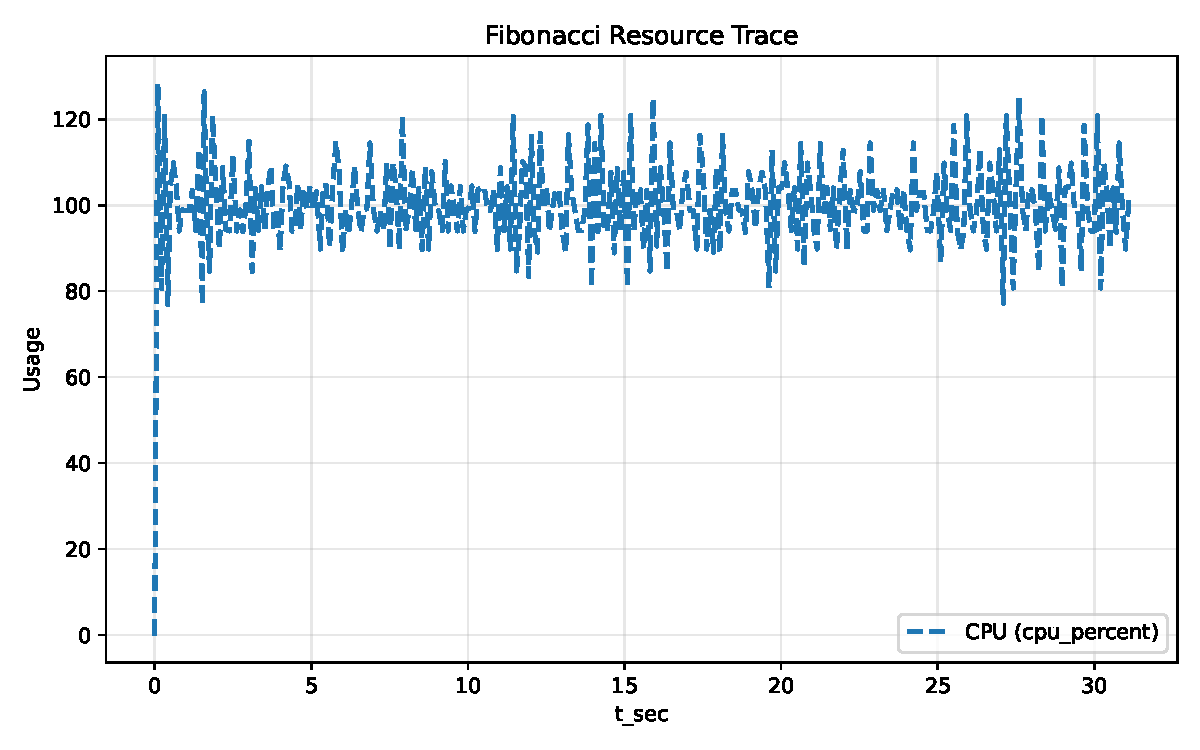
\includegraphics[width=.9\textwidth]{chapters/fib_memprobe_plot.pdf}
  \caption{Observed CPU and memory footprint for naive recursion.
  Exponential calls lead to geometric memory growth.}
  \label{fig:memtrace}
\end{figure}

\subsection{Big-O vs. Reality}
Big-O describes asymptotic shape, not scale. It ignores constants,
compiler optimizations, cache misses, and human sighs. Yet its
\emph{curve} predicts the suffering accurately:
\[
O(2^n) \text{ feels like doubling pain every increment of } n.
\]
Memoization reclaims sanity by converting the chaos to $O(n)$.
The plot in Figure~\ref{fig:bigoreal} overlays theoretical curves
with empirical data—showing that while constants differ, shapes
endure.

\begin{figure}[htbp]
  \centering
  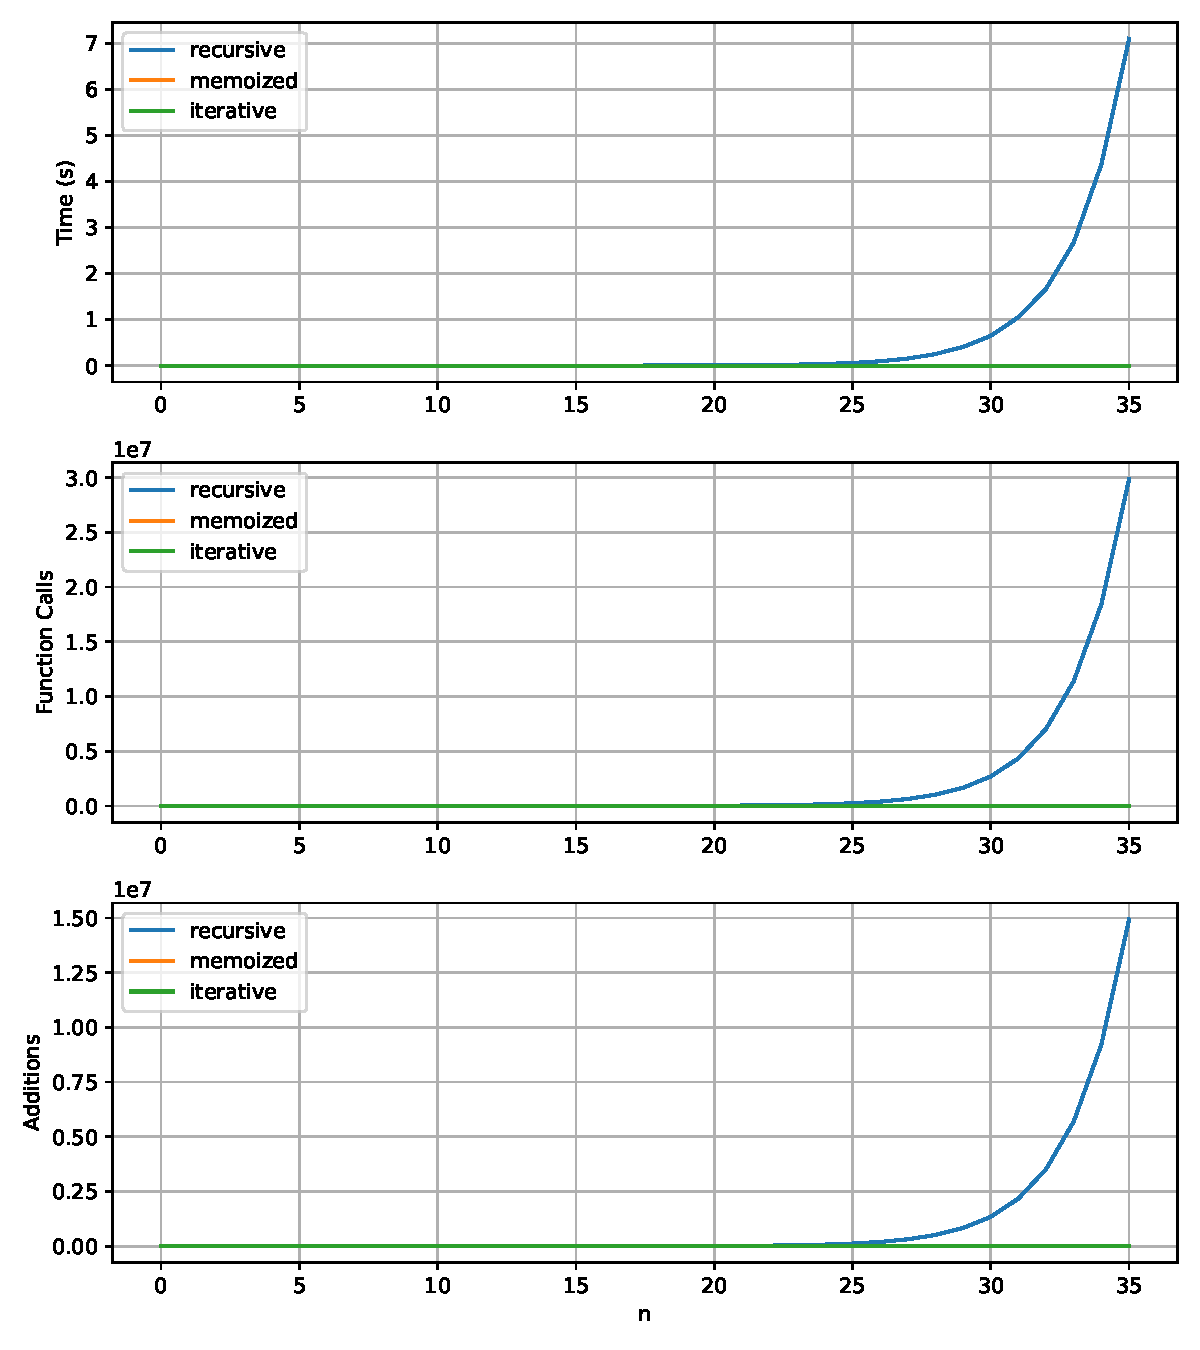
\includegraphics[width=.85\textwidth]{chapters/fib_bench_plot.pdf}
  \caption{Naive recursion (red, $O(2^n)$) vs. memoized (green, $O(n)$).
  Reality hugs the theory.}
  \label{fig:bigoreal}
\end{figure}

\section{Beyond Big-O: When the Stack Runs Out}

The naive recursive Fibonacci is limited not just by time but by
stack depth and heap exhaustion. Past a certain $n$, Python
throws a \texttt{RecursionError}. The cost curve is no longer
mathematical—it is existential.

\begin{quote}
\textbf{Observation:} Big-O assumes infinite memory and patience.
Your laptop does not.
\end{quote}

\section{Reflection Prompts}
\begin{enumerate}
  \item At what $n$ did your system fail or slow dramatically?
  \item Compare your CPU temperature trace to your time complexity plot.
  \item What constant factors made the real data deviate from $2^n$?
  \item How does memoization mimic biological memory in reducing energy waste?
\end{enumerate}

\section{Epilogue: The Shape of Pain}
In this chapter, the curve of $2^n$ became audible—the fans whirred,
the heat rose, the machine groaned. The math foretold it. And that,
dear reader, is the poetry of Big-O.

